
\section{TMTO}

\subsection{a)}
Wir haben festgestellt, dass die Tabelle mit einer größeren Entropie aufgrund von 4 Byte Passwörtern auch größer werden. \\
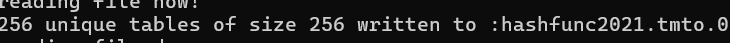
\includegraphics[width=0.7\textwidth]{img/TMTO_24Bit_Größe.png}\\
Hier hatten wir 256 Tabellen unique Tabellen mit 256 Endpuntken.\\
Bei Passwörtern der größe 4 Byte hatten wir dann 1625 unique Tabellen mit 1625 Endpunkten.\\
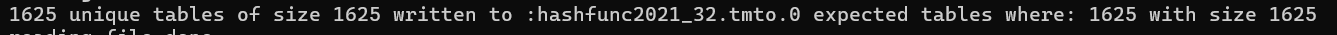
\includegraphics[width=1\textwidth]{img/tmto_32_größe.png}
\subsection{b) Bei TMTO-Angriffen spielt der Parameter N eine zentrale Rolle. Wie groß ist N hier? Wie ist die Aufteilung von Zeilen (m) und Spalten (l) gewählt worden? Warum wurden diese so gewählt?}

\textbf{Satz von Hellmann:}

\noindent Die Erfolgswahrscheinlichkeit liegt bei 80\% (für $N$ groß genug, z.B. $N = 2^{56}$ ), wenn man $1 \leq k \leq \lceil N^\frac{1}{3} \rceil$ unterschiedliche $f_k$ wählt und für jedes $f_k$ eine TMTO-Tabelle mit $n = m = \lceil N^\frac{1}{3} \rceil$ anlegt, als zu einem $f$ eine Tabelle mit $m = \lceil N^\frac{1}{3} \rceil \text{ und } n = \lceil N^\frac{2}{3} \rceil$ zu erzeugen.

Wir haben eine Entropie von 36 Bit. Demnach ist $N = 2^{36}$. Nach dem Satz von Hellmann gilt:
$$
n = m = \lceil N^{\frac{1}{3}} \rceil = \lceil 2^{\frac{36}{3}} \rceil  = 4096
$$
\newpage
\subsection{c) BestimmenSie die Erfolgswahrscheinlichkeit Ihrer Tabelle empirisch für 1000 zufällig gewählte Passwörter. Dazu erzeugen Sie zufällige und einmalige Passwörter, hashen diese und suchen die Hashes in der Tabelle. Dokumentieren Sie Ihr Ergebnis. Vergleichen Sie die Erfolgswahr scheinlichkeit mit den Erwartungswerten von Öchslin und Hellmann. Wiederholen Sie dies auch für 24 Bit, hier allerdings für 1 Mio. zufällige Passwörter. Dokumentieren Sie Ihre Ergebnisse.}

Für unsere erstellte 24Bit Tabelle und 1 Millionen Testfälle haben folgende Coverage erreicht: \\
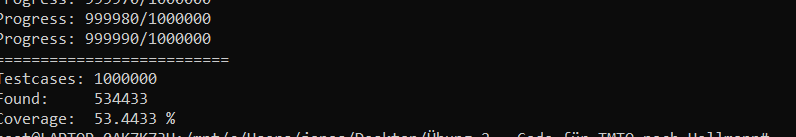
\includegraphics[width=0.7\textwidth]{img/Coverage_24Bit.png}\\
Für unsere 32 Bit Tabelle haben wir eine Coverage von 54,1\% auf 1000 Testwerten\\
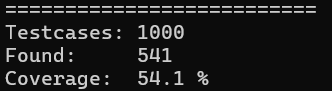
\includegraphics[width=0.7\textwidth]{img/coverage_32bit.png}\\
Auch wenn wir die Aufteilung nach Hellman berechnen, bekommen wir nicht die zu erwartenden 80\% Coverage, aber wir erfüllen auch nicht die Bedingung eines genügend großen N, nämlich mindestens $2^{56}$.
\subsection{d) Wäre der TMTO-Ansatz noch effizient, wenn ein 96 bit langer Salt verwendet wird und wie folgt gehast wird:
$p_1p_2p_3p_4p_5s_1...s_{95}$ werden als $128$ bit Schlüssel K aufgefasst und der Passworthash ist die AES-Verschlüsselung von einem 128-Null-Bit String mit diesem Schlüssel Wie verändert sich die Situation, wenn der Salt immer aus $96$ Nullen besteht. Begründen sie ihre Antwort mathematisch.}

\begin{enumerate}
    \item Bei dem ersten Ansatz ist der TMTO-Ansatz nicht mehr effizient. Die Passwortkomplexität N wird zu $N=2^{128}$ und die Suchzeit wird zu$\mathcal{O}(\log 128 \cdot 2^\frac{128 \cdot 2}{3}) \approx \mathcal{O}(\log 2 \cdot 2^{85})$.
    \item Bei dem zweiten Ansatz hat der Salt kaum Auswirkungen auf die Suchkomplexität. Die Übergangsfunktion der TMTO kann einfach so gewählt werden, dass aus einem gegebenen Hash immer ein Passwort gebildet, dessen Salt-Bits null sind. Dadurch bleibt es bei der Ursprünglichen Komplexität. Allerdings erhöht sich ggf. die Kollisionswahrscheinlichkeit in unserem TMTO-Ansatz.
\end{enumerate}

\subsection{e) Was ist der Unterschied zwischen Salt und Pepper?}
Salt und Pepper sind beides Gegenmaßnahmen, Angriffe auf Datenbanken zu erschweren in denen Passwörter gespeichert sind. Beides sind dabei Werte die auf den Hash draufgerechnet werden mit dem Unterschied das der Salt in der Datenbank selber gespeichert wird und Pepper in einer Externen Datenbank. Der Vorteil von einer Externen Speicherung wie bei Pepper ist dann natürlich, dass wenn die Passwort-Datenbank kompromittiert ist, der Pepper trotzdem noch nicht zugänglich ist.
%Effektiv bei einem Salt der 16 Bit groß ist erhöht sich die Kompletität für TMTO Tabellen von $2^{16}$. Dies ist der Fall da für jedes PW was wir raten und den Hash erzeugen nun auch noch $2^{16}$ verschiedene Salts getestet werden müssen bzw. Gibt es zu jedem Hash weitere $2^{16}$ mögliche enstandene Hashes.

\subsection{f) Nennen Sie mindestens zwei weitere Gegenmaßnahmen für Passwortangriffe mit kurzer Begründung.}
\begin{enumerate}
    \item Es wird eine Hashfunktion gewählt, die effizient genug für seltenes Berechnen, aber ineffizient für mehrfaches Berechnen ist. Angreifer berechnen für gewöhnlich häufiger Hashwerte als Server.
    \item Es wird eine Hashfunktion gewählt, die auf spezialisierter Hardware nicht effizienter zu verwenden ist, als auf herkömmlicher. Dadurch kann man ineffiziente Algorithmen nicht mit der Wahl der Hardware ausgleichen.
\end{enumerate}





